% MATLAB source: paper/plot_existing_manuscript_figures.m
\begin{figure}[htbp]
  \centering
  \begin{subfigure}[t]{0.485\linewidth}
    \centering
    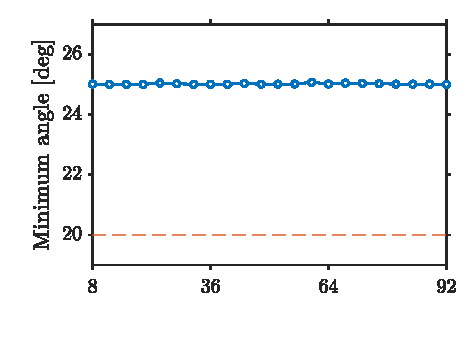
\includegraphics[width=\linewidth]{figures/quality/min_angle.pdf}
    \caption{Minimum triangle-angle check.}
    \label{fig:quality-angle}
  \end{subfigure}
  \hfill
  \begin{subfigure}[t]{0.485\linewidth}
    \centering
    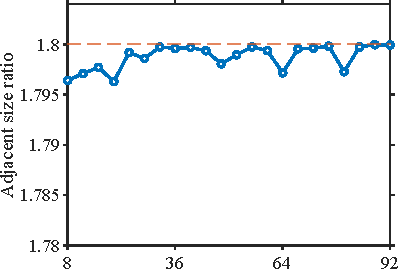
\includegraphics[width=\linewidth]{figures/quality/size_ratio.pdf}
    \caption{Adjacent element-size-ratio check.}
    \label{fig:quality-ratio}
  \end{subfigure}

  \medskip

  \begin{subfigure}[t]{0.485\linewidth}
    \centering
    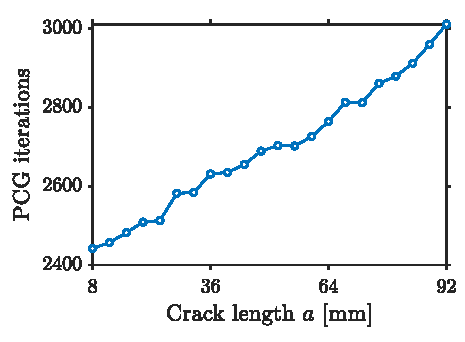
\includegraphics[width=\linewidth]{figures/quality/iterations.pdf}
    \caption{PCG iterations for accepted physical solves.}
    \label{fig:quality-iterations}
  \end{subfigure}
  \hfill
  \begin{subfigure}[t]{0.485\linewidth}
    \centering
    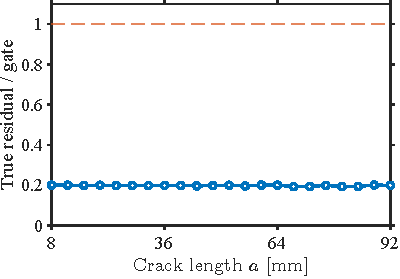
\includegraphics[width=\linewidth]{figures/quality/true_residual.pdf}
    \caption{True relative residual normalized by its acceptance gate.}
    \label{fig:quality-residual}
  \end{subfigure}

  \caption{Diagnostics for accepted $P_2$--$P_{23}$ states. Dashed lines are
  the $20^\circ$ minimum-angle gate, 1.8 adjacent-size-ratio gate, and normalized
  true-residual gate of one. The separately enforced reported-PCG tolerance
  is $10^{-10}$; the true-residual acceptance denominator is
  $5\times10^{-10}$. No failed $P_{24}$ solve is plotted.}
  \label{fig:quality}
\end{figure}
